\section*{Problem 1 - Attitude Control of Satellite}



\subsection*{Problem 1.1} 

\begin{equation}
\label{eq:dynamics}		% The label is used when referring to this equation. 
	\begin{aligned}
		\dot{\mathbf{q}} = \mathbf{T}_q (\mathbf{q} ) \boldsymbol{\omega} \\
		\mathbf{I}_{CG} \dot{\boldsymbol{\omega}} - \mathbf{S} (\mathbf{I}_{CG} \boldsymbol{\omega} ) \boldsymbol{\omega} & =  \boldsymbol{\tau}
	\end{aligned}	
\end{equation}

Rewriting equation \ref{eq:dynamics}, we can find the equilibrium points for the Sattelite system by solving equation \ref{eq:dynamics2} given the  initial values. 

\begin{equation}
\label{eq:dynamics2}		% The label is used when referring to this equation. 
	\begin{aligned}
		\dot{\mathbf{q}} = \mathbf{T}_q (\mathbf{q} ) \boldsymbol{\omega} \\
		\dot{\boldsymbol{\omega}} =  \frac{1}{\mathbf{I}_{CG}} (\boldsymbol{\tau} + \mathbf{S} (\mathbf{I}_{CG} \boldsymbol{\omega} ) \boldsymbol{\omega} &)
	\end{aligned}	
\end{equation}

\begin{equation}
    \begin{bmatrix}
        \dot{\varepsilon}_1 \\ \dot{\varepsilon}_2 \\ \dot{\varepsilon}_3
    \end{bmatrix}
    = \frac{1}{2}
      \begin{bmatrix}
        \eta & -\varepsilon_3 & \varepsilon_2 \\ \varepsilon_3 & \eta & - \varepsilon_1 \\ -\varepsilon_2 & \varepsilon_1 & \eta
    \end{bmatrix} 
    \omega
\end{equation}

\begin{equation}
    \begin{bmatrix}
    \dot{p} \\ \dot{q} \\ \dot{r}
    \end{bmatrix}
    =
    \begin{bmatrix}
    \frac{\tau_1}{mR^2} \\ \frac{\tau_2}{mR^2} \\ \frac{\tau_3}{mR^2} 
    \end{bmatrix}
\end{equation}




Inserting the initial values into equations 3 and 4, the calculated equilibrium points become the following: 
\begin{align*}
    \mathbf{x}_0 =
    \begin{bmatrix}
        \varepsilon_1 \\ \varepsilon_2 \\ \varepsilon_3 \\p \\ q \\ r 
    \end{bmatrix}
    = 
    \begin{bmatrix}
        0 \\ 0 \\ 0 \\ 0 \\ 0 \\ 0
    \end{bmatrix}
\end{align*}

Linearizing the spacecraft model around $x_0$: 

\begin{equation}
    \dot{\mathbf{x}} = \mathbf{f(x)}
    \begin{bmatrix}
        \frac{1}{2}(\eta \mathbf{p} -\varepsilon_3 \mathbf{q} + \varepsilon_2 \mathbf{r}) \\
        \frac{1}{2}(\varepsilon_3 \mathbf{p} + \eta \mathbf{q}  - \varepsilon_1 \mathbf{r})\\
        \frac{1}{2}(-\varepsilon_2 \mathbf{p} +\varepsilon_1 \mathbf{q} + \eta \mathbf{r}) \\
        \frac{\tau_1}{mR^2}\\
        \frac{\tau_2}{mR^2}\\
        \frac{\tau_3}{mR^2}\\
    \end{bmatrix} 
\end{equation}


\begin{equation}
    \dot{x} = \frac{df}{dx_{|x_0}}(x-x_0) + \frac{df}{du_{|u_0}}(u-u_0)
\end{equation}

Calculating the jacobians with the initial values results in the linearized model:

\begin{equation}
    \dot{x} = 
    \begin{bmatrix}
        0 & 0 & 0 & \frac{1}{2}  & 0 & 0 \\
        0 & 0 & 0 & 0 & \frac{1}{2}  & 0 \\
        0 & 0 & 0 & 0 & 0 & \frac{1}{2}  \\
        0 & 0 & 0 & 0 & 0 & 0 \\
        0 & 0 & 0 & 0 & 0 & 0 \\
        0 & 0 & 0 & 0 & 0 & 0 \\
    \end{bmatrix}
    x + 
    \begin{bmatrix}
        0 & 0 & 0 \\
        0 & 0 & 0 \\
        0 & 0 & 0 \\
        \frac{1}{720} & 0 & 0 \\
        0 & \frac{1}{720}  & 0 \\
        0 & 0 & \frac{1}{720} \\
    \end{bmatrix}
    u
\end{equation}








\subsection*{Problem 1.2}

The linearized system can be written like this. 

\begin{align*}
A_{ol} &= \begin{bmatrix}
    \mathbf{0}_{3\times3} & \mathbf{I}_{3\times3} \\
    \mathbf{0}_{3\times3} & \mathbf{0}_{3\times3}
\end{bmatrix}; \\
B &= \begin{bmatrix}
    \mathbf{0}_{3\times3} \\
    \mathbf{I}_{\text{inv}}
\end{bmatrix}; \\
K &= \begin{bmatrix}
    kp\cdot\mathbf{I}_{3\times3} & kd\cdot\mathbf{I}_{3\times3}
\end{bmatrix}; \\
A_{cl} &= A_{ol} - B\cdot K
\end{align*}

where $A_{ol}$ and $A_{cl}$ are the open loop and closed loop system matrices respectively. 

The eigenvalues of the closed-loop system are:
\begin{align*}
&-0.0278 + 0.0448i \\
&-0.0278 - 0.0448i \\
&-0.0278 + 0.0448i \\
&-0.0278 - 0.0448i \\
&-0.0278 + 0.0448i \\
&-0.0278 - 0.0448i
\end{align*}

All poles are located in the left half plane, so the closed loop system is stable. 

The system should have critical damping avoiding oscillations of the satellite, which means that we want strictly real poles. 


\subsection*{Problem 1.3}
% Answer Problem 1.3 here. Equation (2) from the assignment can be written as: 
% \begin{equation}
%   \label{eq:tau}
%   \mathbf{\tau} = -\mathbf{K}_d \boldsymbol{\omega} - k_p \boldsymbol{\varepsilon}
% \end{equation}

\begin{figure}
    \centering
    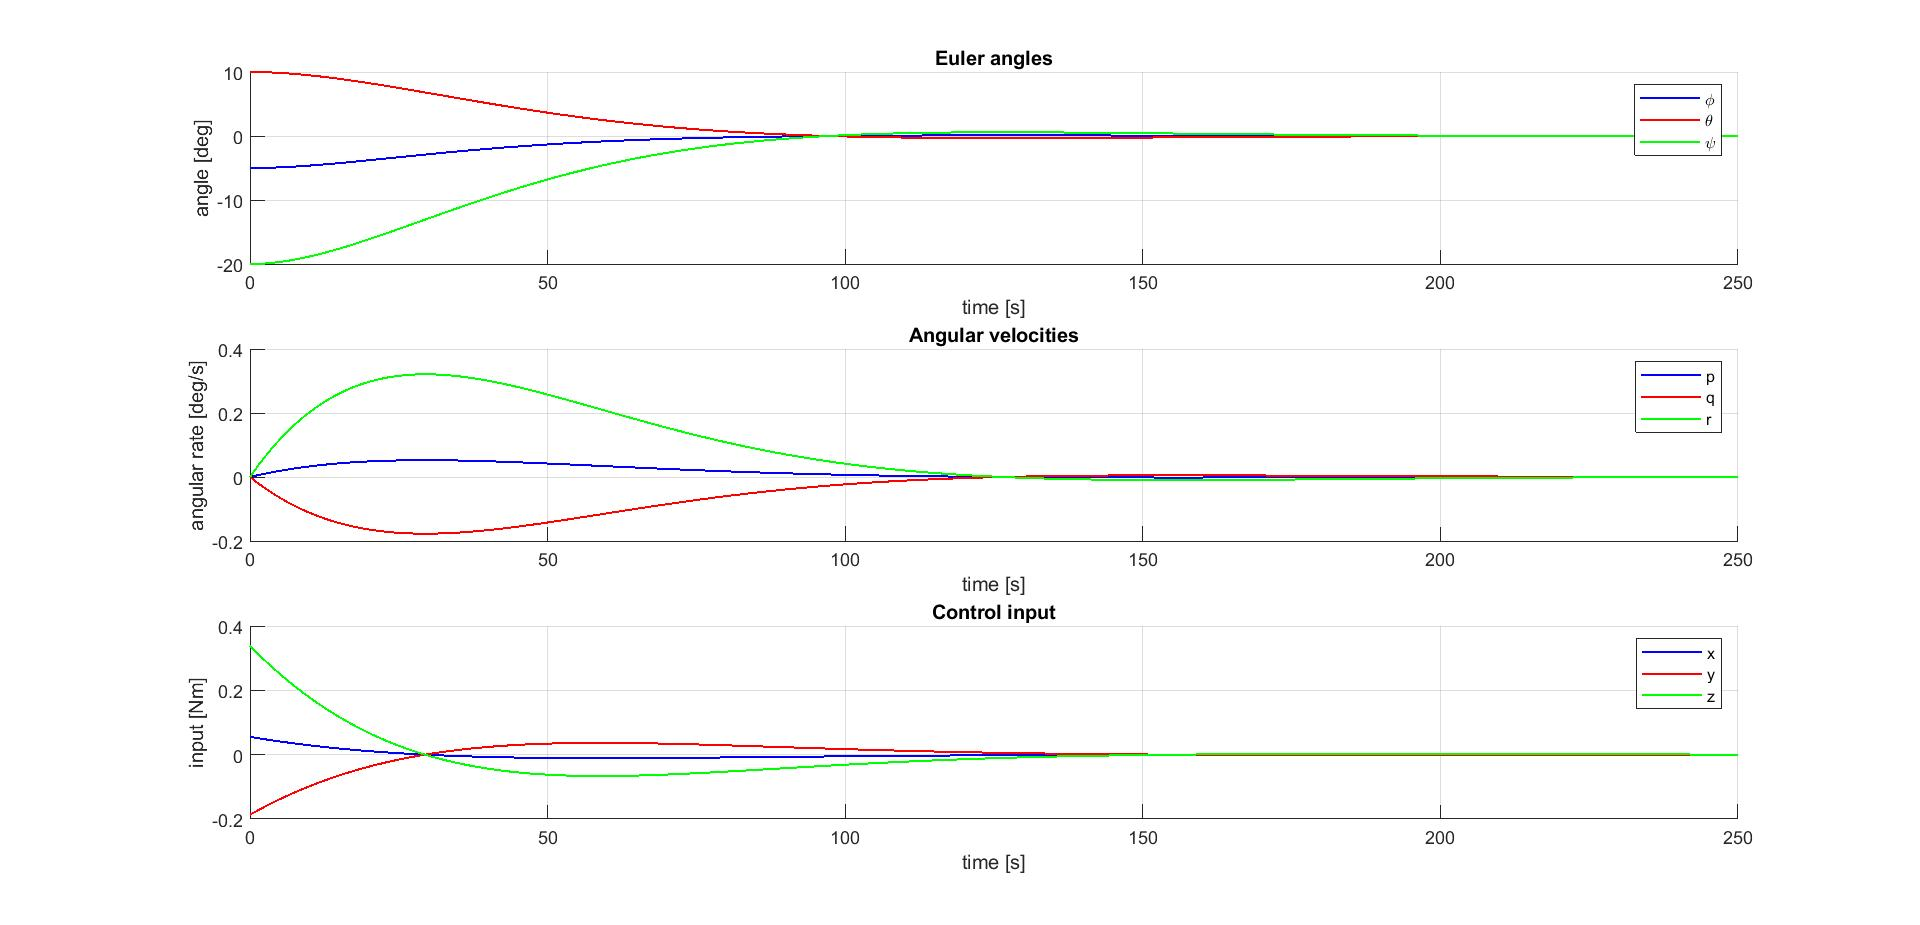
\includegraphics[width=1\textwidth]{figures/task1_3.jpg}
    \caption{Setpoint regulation with zero reference}
    \label{fig:task13}
\end{figure}

The system matches our expectations, as shown in figure \ref{fig:task13}. All states go to zero. This is expected since the system is stable, and there is no feed forward term. There are some oscillations due to the non zero imaginary parts of the eigenvalues. 
The control input also goes to zero, as a should since its is proportional to the state vector. 

In order to follow nonzero constant reference signals We  modify the control law so that we control the state error to zero, in stead of the state. 
Since the we have a constant reference signal, $w_d$ is zero, so no modification is required. When defining the error of the angels, we cannot subtract $q$ from $q_d$
since quaternions are not closed under subtraction. In stead we use the definition given in task 1.4.

\subsection*{Problem 1.4}
The quaternion error can be written as
 \begin{equation}
	 \tilde{\mathbf{q}} := \left[
	 \begin{array}{c}
		 \tilde{\eta} \\
		 \tilde{\varepsilon}
	 \end{array}
	 \right] = \bar{\mathbf{q}}_d \otimes \mathbf{q} 
 \end{equation}

\begin{equation}
    \tilde{\mathbf{q}} = 
    \begin{bmatrix}
        \sqrt{1-(\varepsilon^2_{1d} + \varepsilon^2_{1d} +\varepsilon^2_{1d})} 
        \sqrt{1-(\varepsilon^2_{1} + \varepsilon^2_{1} +\varepsilon^2_{1})}
        + \varepsilon_{1d}\varepsilon_{1} + \varepsilon_{2d}\varepsilon_{2} + \varepsilon_{1d}\varepsilon_{1d} \\
        \sqrt{1-(\varepsilon^2_{1d} + \varepsilon^2_{1d} +\varepsilon^2_{1d})} \varepsilon_1 -
        \sqrt{1-(\varepsilon^2_{1d} + \varepsilon^2_{1d} 
        +\varepsilon^2_{1d})} \varepsilon_{1d} 
        -\varepsilon_{2d}\varepsilon_{3} + 
        \varepsilon_{3d}\varepsilon_{2}\\
        \sqrt{1-(\varepsilon^2_{1d} + \varepsilon^2_{1d} +\varepsilon^2_{1d})} \varepsilon_2 -
        \sqrt{1-(\varepsilon^2_{1d} + \varepsilon^2_{1d} 
        +\varepsilon^2_{1d})} \varepsilon_{2d} 
        +\varepsilon_{1d}\varepsilon_{3}
        -\varepsilon_{3d}\varepsilon_{1}
        \\
        \sqrt{1-(\varepsilon^2_{1d} + \varepsilon^2_{1d} +\varepsilon^2_{1d})} \varepsilon_3 -
        \sqrt{1-(\varepsilon^2_{1d} + \varepsilon^2_{1d} +\varepsilon^2_{1d})} \varepsilon_{3d}
        -\varepsilon_{1d}\varepsilon_{2}
        +\varepsilon_{2d}\varepsilon_{1}
        
    \end{bmatrix}
\end{equation} 

When the reference is constant, the variable $q$ converges toward $q_d$ due to the influence of negative feedback control. Furthermore, assuming that $q$ has converged to $q_d$, we can observe that $\tilde q = q_d\otimes q_d = [1, 0, 0, 0]^\top$. Here the imaginary part of the quaternion $\varepsilon$, equals zero. This convergence makes sense since the quaternion has no imaginary part when the error is zero, which aligns with the objective of the PD controller's error minimization.

\subsection*{Problem 1.5}

\begin{figure}[ht]
	\centering
	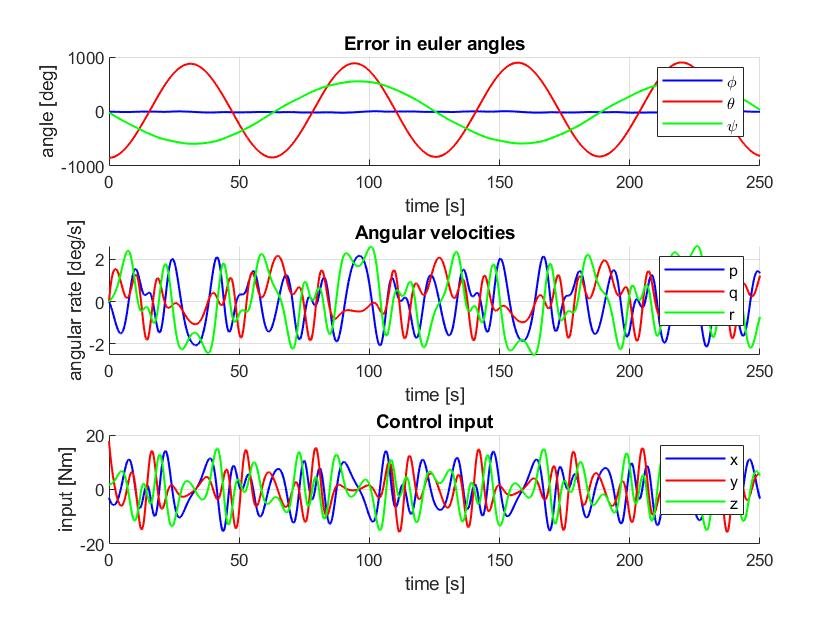
\includegraphics[width=1\textwidth]{figures/task1_5.jpg} 
	\caption{Using time varying reference signals.}
	\label{fig:task15}
\end{figure}

\begin{figure}[ht]
	\centering
	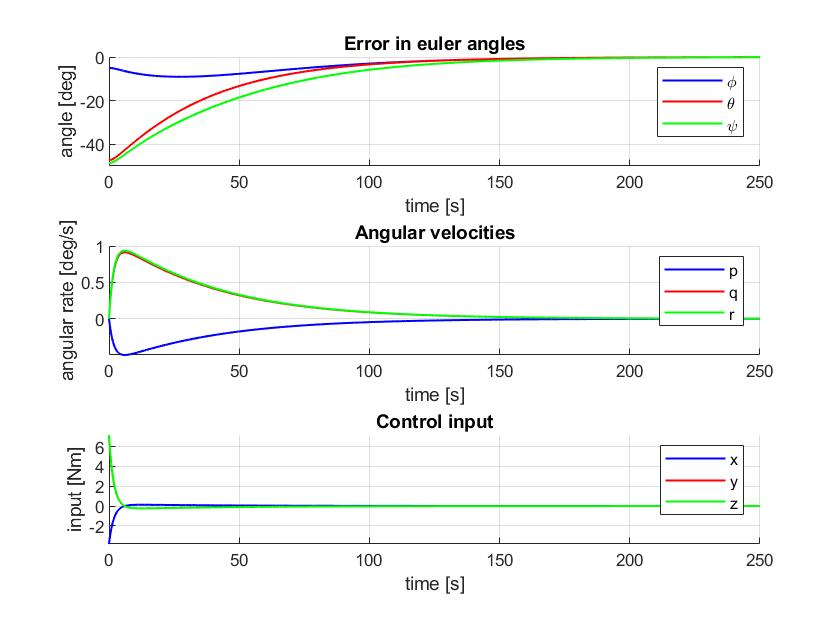
\includegraphics[width=1\textwidth]{figures/task1_5const.jpg} 
	\caption{Using constant reference signals different from zero.}
	\label{fig:task15const}
\end{figure}

The controller is not capable of following the reference signal, as seen in fig \ref{fig:task15}. This is logic since we are trying to control angular velocity towards zero, while simultaneously control the angels towards varying references. The angular velocity should be controlled towards the time derivative of the reference signal. 
Figure \ref{fig:task15const} demonstrates the the controller is capable of controlling the system to a reference different from zero, the the time derivative of the reference signal is zero. 



\subsection*{Problem 1.6}
The control law in this problem can be written as
\begin{equation}
	\boldsymbol{\tau} = -\mathbf{K}_d \tilde{\boldsymbol{\omega}} - k_p \tilde{\boldsymbol{\varepsilon}}
\end{equation}
and the desired angular velocity as
\begin{equation}
	\boldsymbol{\omega}_d = \mathbf{T}^{-1}_{\Theta_d}(\Theta_d)\dot{\Theta}_d
\end{equation}

We expected that this controller would outperform the one used in task 1.5, because the angular velocity is now regulated towards the time derivative of the target signal. It does so nicely, as seen in \autoref{fig:task1_6}. 


\begin{figure}[ht]
	\centering
	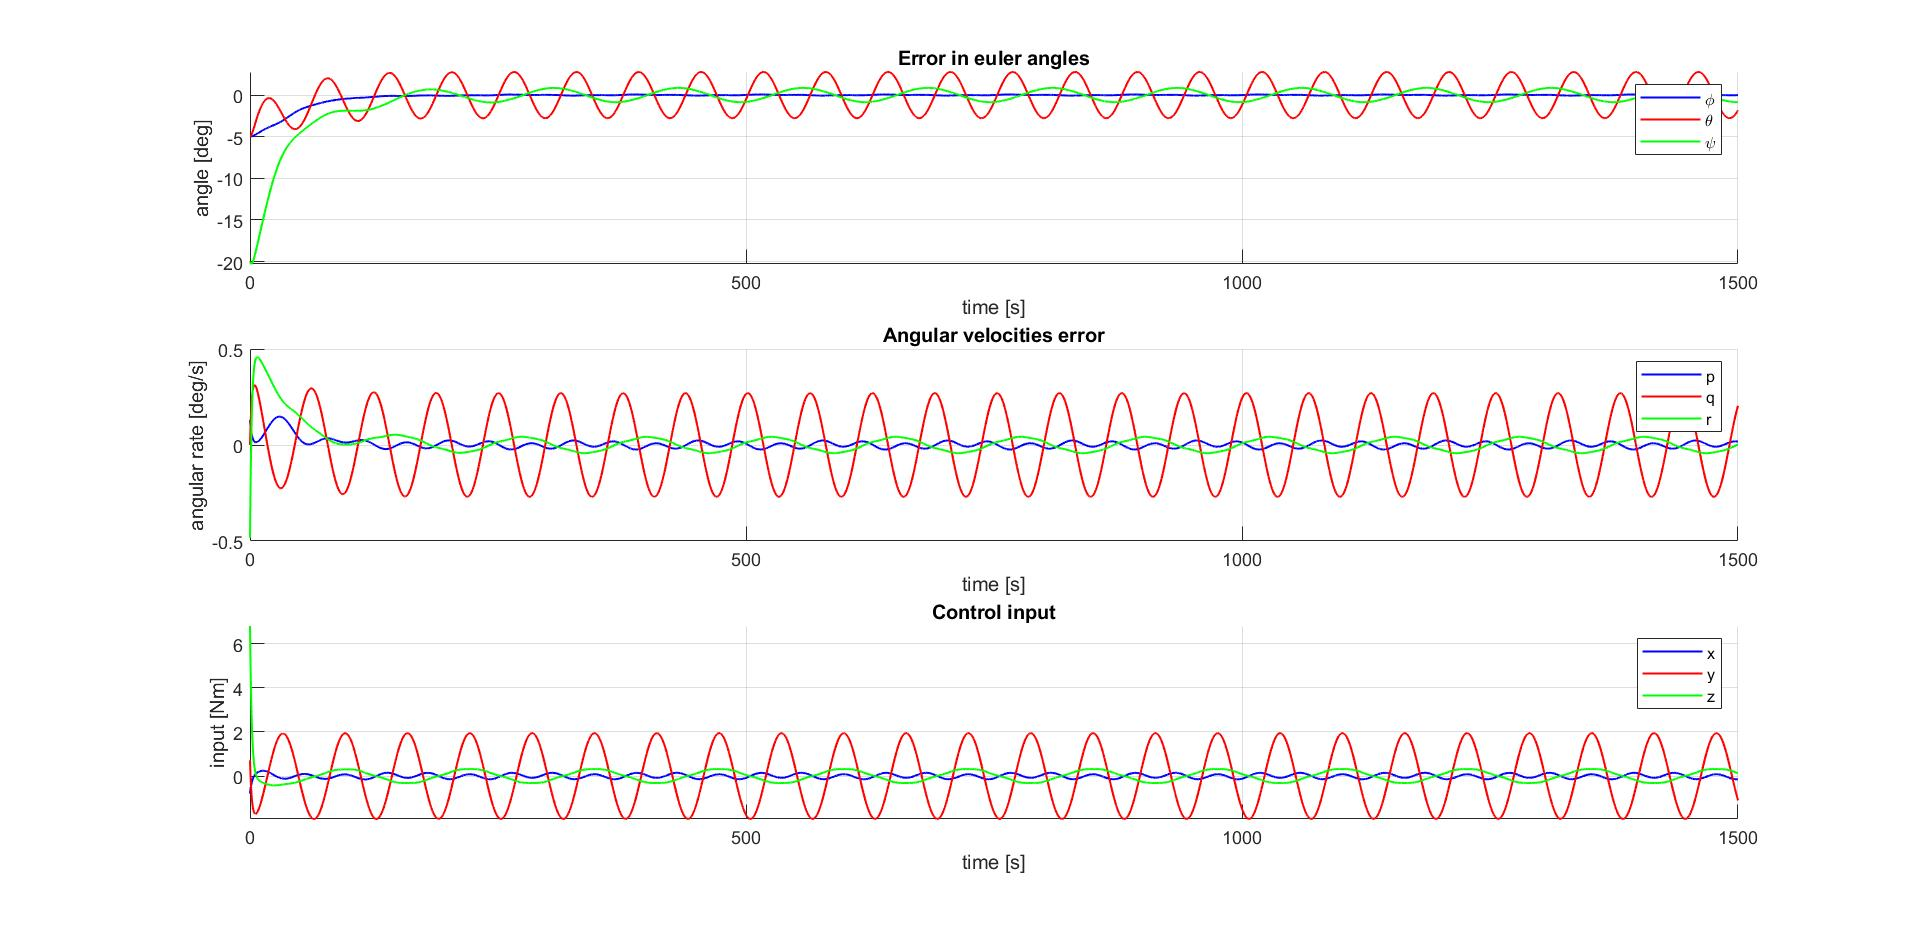
\includegraphics[width=1\textwidth]{figures/task1_6.jpg} 
	\caption{Using time varying reference signals for both angle and angular velocity.}
	\label{fig:task16}
\end{figure}

\subsection*{Problem 1.7}
\subsubsection*{a)}
The Lyapunov function can be written as 
 \begin{equation}
	 V = \frac{1}{2} \tilde{\boldsymbol{\omega}}^{\top} \mathbf{I}_{CG}\tilde{\boldsymbol{\omega}} + 2 k_p (1-\tilde{\eta})
 \end{equation}
and the derivative as 
\begin{equation}
	\dot{V} = -k_d \omega^{\top} \mathbf{I_g} \dot\omega
 + 2\mathbf{k_P}(-\dot\eta)
\end{equation}

\begin{equation}
	\dot{V} = \omega^{\top}\mathbf{I_g}\mathbf{I_g}^{-1}(\mathbf{S}(\mathbf{I_g}\omega)\omega-\mathbf{k_d}\omega
 -\mathbf{k_p}\varepsilon + \mathbf{k_p}\varepsilon^{\top}\omega
\end{equation}

\begin{equation}
	\dot{V} = \omega^{\top}\mathbf{I_g}\mathbf{I_g}^{-1}(\mathbf{S}(\mathbf{I_g}\omega)\omega-\mathbf{k_d}\omega
 -\mathbf{k_p}\varepsilon + \mathbf{k_p}\varepsilon^{\top}\omega
\end{equation}


\begin{equation}
	\dot{V} = \omega^{\top}(\mathbf{S}(\mathbf{I_g}\omega)\omega-\omega^{\top}\mathbf{k_d}\omega
 -\omega^{\top}\mathbf{k_p}\varepsilon + \mathbf{k_p}\varepsilon^{\top}\omega
\end{equation}

\begin{equation}
	\dot{V} = -\omega^{\top}\mathbf{k_d}\omega
\end{equation}


\subsubsection*{b)}
We have that:
\begin{enumerate}
    \item The Lyaponov function in equation (9) is continuously differentiable and positive definite.
    \item It is radially unbounded. This is clear since $\varepsilon$ grow when $\eta$ grows.
    \item The derivative of the Lyaponov function given in (10) is negative semi definite. 
\end{enumerate} 
Thus we can use Karzovskii-LaSalle's theorem. 

We have $\Omega = \{\omega=0\}$. 
The largest invariant set $M$ within $\Omega$, is all solutions of $\dot{x} = 0$ with $\omega=0$. 
We get $M=\{w=0, \varepsilon=\varepsilon_0\}=\{x_{equilibrium}\}$.  Thus we can conclude that the equilibrium of the closed-loop system is asymptotically stable.

\subsubsection*{c)}
Two different quaternions represent the same angle. Thus there are two equilibriums. Thus global asymptotic stability is impossible. 